%%%%%%%%%%%%%%%%%%%%%%%%%%%%%%%%%%%%%%%%%
% Beamer Presentation
% LaTeX Template
% Version 2.0 (March 8, 2022)
%
% This template originates from:
% https://www.LaTeXTemplates.com
%
% Author:
% Vel (vel@latextemplates.com)
%
% License:
% CC BY-NC-SA 4.0 (https://creativecommons.org/licenses/by-nc-sa/4.0/)
%
%%%%%%%%%%%%%%%%%%%%%%%%%%%%%%%%%%%%%%%%%

%----------------------------------------------------------------------------------------
%	PACKAGES AND OTHER DOCUMENT CONFIGURATIONS
%----------------------------------------------------------------------------------------

\documentclass[
	12pt, % Set the default font size, options include: 8pt, 9pt, 10pt, 11pt, 12pt, 14pt, 17pt, 20pt
	%t, % Uncomment to vertically align all slide content to the top of the slide, rather than the default centered
	%aspectratio=169, % Uncomment to set the aspect ratio to a 16:9 ratio which matches the aspect ratio of 1080p and 4K screens and projectors
]{beamer}

\graphicspath{{Images/}{./}} % Specifies where to look for included images (trailing slash required)

\usepackage{booktabs} % Allows the use of \toprule, \midrule and \bottomrule for better rules in tables

\usepackage[dvipsnames]{xcolor}
%----------------------------------------------------------------------------------------
%	SELECT LAYOUT THEME
%----------------------------------------------------------------------------------------

% Beamer comes with a number of default layout themes which change the colors and layouts of slides. Below is a list of all themes available, uncomment each in turn to see what they look like.

%\usetheme{default}
%\usetheme{AnnArbor}
%\usetheme{Antibes}
%\usetheme{Bergen}
%\usetheme{Berkeley}
%\usetheme{Berlin}
\usetheme{Boadilla}
%%%%%%%%%\usetheme{CambridgeUS}
%\usetheme{Copenhagen}
%\usetheme{Darmstadt}
%\usetheme{Dresden}
%\usetheme{Frankfurt}
%\usetheme{Goettingen}
%\usetheme{Hannover}
%\usetheme{Ilmenau}
%\usetheme{JuanLesPins}
%\usetheme{Luebeck}
%%%%%\usetheme{Madrid}
%\usetheme{Malmoe}
%\usetheme{Marburg}
%\usetheme{Montpellier}
%\usetheme{PaloAlto}
%\usetheme{Pittsburgh}
%\usetheme{Rochester}
%\usetheme{Singapore}
%\usetheme{Szeged}
%\usetheme{Warsaw}

%----------------------------------------------------------------------------------------
%	SELECT COLOR THEME
%----------------------------------------------------------------------------------------

% Beamer comes with a number of color themes that can be applied to any layout theme to change its colors. Uncomment each of these in turn to see how they change the colors of your selected layout theme.

%\usecolortheme{albatross}
\usecolortheme{beaver}
%\usecolortheme{beetle}
%\usecolortheme{crane}
%\usecolortheme{dolphin}
%\usecolortheme{dove}
%\usecolortheme{fly}
%%%%%%%%\usecolortheme{lily}
%\usecolortheme{monarca}
%\usecolortheme{seagull}
%\usecolortheme{seahorse}
%\usecolortheme{spruce}
%\usecolortheme{whale}
%\usecolortheme{wolverine}

%----------------------------------------------------------------------------------------
%	SELECT FONT THEME & FONTS
%----------------------------------------------------------------------------------------

% Beamer comes with several font themes to easily change the fonts used in various parts of the presentation. Review the comments beside each one to decide if you would like to use it. Note that additional options can be specified for several of these font themes, consult the beamer documentation for more information.

\usefonttheme{default} % Typeset using the default sans serif font
%\usefonttheme{serif} % Typeset using the default serif font (make sure a sans font isn't being set as the default font if you use this option!)
%\usefonttheme{structurebold} % Typeset important structure text (titles, headlines, footlines, sidebar, etc) in bold
%\usefonttheme{structureitalicserif} % Typeset important structure text (titles, headlines, footlines, sidebar, etc) in italic serif
%\usefonttheme{structuresmallcapsserif} % Typeset important structure text (titles, headlines, footlines, sidebar, etc) in small caps serif

%------------------------------------------------

%\usepackage{mathptmx} % Use the Times font for serif text
\usepackage{palatino} % Use the Palatino font for serif text

%\usepackage{helvet} % Use the Helvetica font for sans serif text
\usepackage[default]{opensans} % Use the Open Sans font for sans serif text
%\usepackage[default]{FiraSans} % Use the Fira Sans font for sans serif text
%\usepackage[default]{lato} % Use the Lato font for sans serif text
\definecolor{grayhover}{rgb}{0.5, 0.5, 0.5}
%----------------------------------------------------------------------------------------
%	SELECT INNER THEME
%----------------------------------------------------------------------------------------

% Inner themes change the styling of internal slide elements, for example: bullet points, blocks, bibliography entries, title pages, theorems, etc. Uncomment each theme in turn to see what changes it makes to your presentation.

%\useinnertheme{default}
\useinnertheme{circles}
%\useinnertheme{rectangles}
%\useinnertheme{rounded}
%\useinnertheme{inmargin}

%----------------------------------------------------------------------------------------
%	SELECT OUTER THEME
%----------------------------------------------------------------------------------------

% Outer themes change the overall layout of slides, such as: header and footer lines, sidebars and slide titles. Uncomment each theme in turn to see what changes it makes to your presentation.

\useoutertheme{default}
%\useoutertheme{infolines}
%\useoutertheme{miniframes}
%\useoutertheme{smoothbars}
%\useoutertheme{sidebar}
%\useoutertheme{split}
%\useoutertheme{shadow}
%\useoutertheme{tree}
%\useoutertheme{smoothtree}

%\setbeamertemplate{footline} % Uncomment this line to remove the footer line in all slides
%\setbeamertemplate{footline}[page number] % Uncomment this line to replace the footer line in all slides with a simple slide count

%\setbeamertemplate{navigation symbols}{} % Uncomment this line to remove the navigation symbols from the bottom of all slides

%----------------------------------------------------------------------------------------
%	PRESENTATION INFORMATION
%----------------------------------------------------------------------------------------

\title[A Fast Low-Level Error Detection Technique]{A Fast Low-Level Error Detection Technique} % The short title in the optional parameter appears at the bottom of every slide, the full title in the main parameter is only on the title page

\subtitle{Zhengyang He, Hui Xu, Guanpeng Li} % Presentation subtitle, remove this command if a subtitle isn't required

\author[Reza Adinepour]{Reza Adinepour} % Presenter name(s), the optional parameter can contain a shortened version to appear on the bottom of every slide, while the main parameter will appear on the title slide

\institute[AUT]{Amirkabir University of Technology\\ (Tehran Polytechnic) \\ \smallskip } % Your institution, the optional parameter can be used for the institution shorthand and will appear on the bottom of every slide after author names, while the required parameter is used on the title slide and can include your email address or additional information on separate lines

\date[\today]{Computer Engineering Department \\ \today} % Presentation date or conference/meeting name, the optional parameter can contain a shortened version to appear on the bottom of every slide, while the required parameter value is output to the title slide

%----------------------------------------------------------------------------------------

\begin{document}

%----------------------------------------------------------------------------------------
%	TITLE SLIDE
%----------------------------------------------------------------------------------------

\begin{frame}
	\titlepage % Output the title slide, automatically created using the text entered in the PRESENTATION INFORMATION block above
	\centering
\includegraphics[scale=0.15]{Images/Logo/logo2.png}
\end{frame}

%----------------------------------------------------------------------------------------
%	TABLE OF CONTENTS SLIDE
%----------------------------------------------------------------------------------------

% The table of contents outputs the sections and subsections that appear in your presentation, specified with the standard \section and \subsection commands. You may either display all sections and subsections on one slide with \tableofcontents, or display each section at a time on subsequent slides with \tableofcontents[pausesections]. The latter is useful if you want to step through each section and mention what you will discuss.

\begin{frame}
	\frametitle{Agenda} % Slide title, remove this command for no title
	
	\tableofcontents % Output the table of contents (all sections on one slide)
	%\tableofcontents[pausesections] % Output the table of contents (break sections up across separate slides)
\end{frame}



%----------------------------------------------------------------------------------------
%	PRESENTATION BODY SLIDES
%----------------------------------------------------------------------------------------

\section{Introduction} % Sections are added in order to organize your presentation into discrete blocks, all sections and subsections are automatically output to the table of contents as an overview of the talk but NOT output in the presentation as separate slides

%------------------------------------------------
%\subsection{Road Map}
%\begin{frame}
%	\frametitle{Road Map}
%	
%	\begin{itemize}
%		\item \textbf{Problem:} Shrinking transistor sizes lead to an increased soft error rate in computer systems, posing a significant risk of severe failures.
%		
%		
%		\item \textbf{Solution:} Introduce Error Detection by Duplicating Instruction (EDDI) at the assembly level.
%		
%		\item \textbf{Main Contribution:}
%		\begin{itemize}
%			\item FERRUM: An enhanced version of EDDI using SIMD and compiler optimizations.
%			\item 100\% fault coverage at the assembly level.
%			\item Over 50\% reduction in runtime overhead compared to existing techniques.
%		\end{itemize}
%	\end{itemize}
%	
%\end{frame}

%------------------------------------------------
\subsection{Problem \& Solutions Overview}
\begin{frame}
	\frametitle{Problem \& Solutions Overview}
	
	\begin{itemize}
		\item \textbf{Problem:}
		Transient hardware faults (soft errors) due to shrinking transistor sizes and operating voltages.
		
		\item \textbf{Impact:}
		Soft errors can cause Silent Data Corruptions (SDCs), compromising system dependability.
		
		\item \textbf{Solutions:}
		\begin{enumerate}
			\item Traditional: Hardware-based methods such as:
			\begin{itemize}
				\item voltage guard bands
				\item redundancy
			\end{itemize}
			\textcolor{red}{have high overhead in performance and energy consumption.}
			
			\item Software-Based: Error Detection by Duplicating Instructions (EDDI)\\
			\textcolor{Green}{has been proposed as a flexible, resource-efficient alternative.}
		\end{enumerate}
	\end{itemize}
\end{frame}

%------------------------------------------------

\subsection{EDDI Methods}
\begin{frame}
	\frametitle{EDDI Methods}
	
	\begin{itemize}
		\item \textbf{EDDI:} 
		Duplicates instructions at compile time and checks for mismatches at runtime.
		
		
		\begin{figure}
			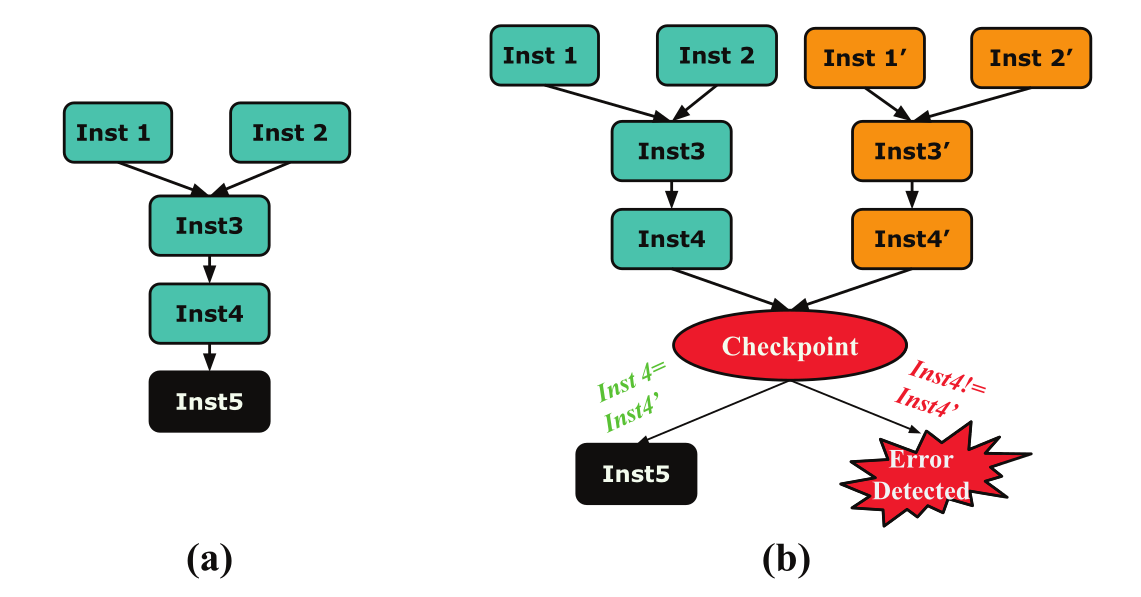
\includegraphics[width=0.9\linewidth]{img1.png}
			\caption{High-level idea of EDDI}
			\label{High-level idea of EDDI}
		\end{figure}
	\end{itemize}
	
	
	
	
	
	
%	\begin{block}{Block Title}
%		Lorem ipsum dolor sit amet, consectetur adipiscing elit. Integer lectus nisl, ultricies in feugiat rutrum, porttitor sit amet augue.
%	\end{block}
%	
%	\begin{exampleblock}{Example Block Title}
%		Aliquam ut tortor mauris. Sed volutpat ante purus, quis accumsan.
%	\end{exampleblock}
%	
%	\begin{alertblock}{Alert Block Title}
%		Pellentesque sed tellus purus. Class aptent taciti sociosqu ad litora torquent per conubia nostra, per inceptos himenaeos.
%	\end{alertblock}
%	
%	\begin{block}{} % Block without title
%		Suspendisse tincidunt sagittis gravida. Curabitur condimentum, enim sed venenatis rutrum, ipsum neque consectetur orci.
%	\end{block}
\end{frame}





% \subsection{EDDI Methods (Cont.)}
\begin{frame}
	\frametitle{EDDI Methods (Cont.)}
	\begin{itemize}
		\item \textbf{Existing EDDI Methods:}
		\begin{enumerate}
			\item Mostly at IR level
		\end{enumerate}
		\textcolor{red}{reduced fault coverage when tested at the assembly level.}
		
		\item \textbf{Problem with IR-Level EDDI:}
		\begin{itemize}
			\item Fault coverage gaps at IR level.
			\item Reduced effectiveness when evaluated at assembly level.
			\item Underestimated error detection at lower levels.
			\item Need for assembly-level implementation for better fault protection.
		\end{itemize}
	\end{itemize}
\end{frame}



%\subsection{Example Code}
\begin{frame}
	\frametitle{IR Code Example Using EDDI}
	
	
	\begin{columns}[c]
		\begin{column}{0.5\textwidth} % Left column width
			\begin{figure}
				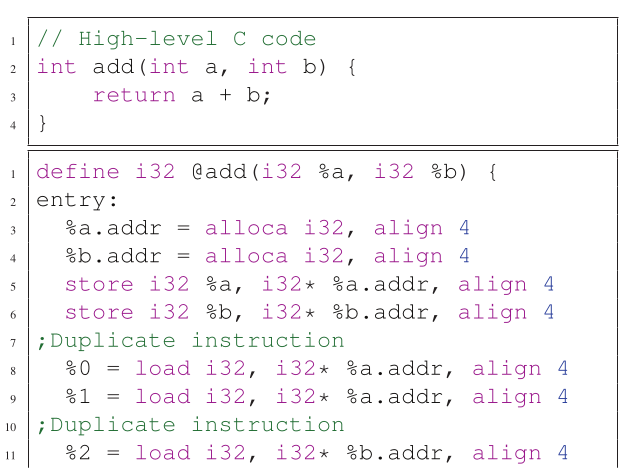
\includegraphics[width=1\linewidth]{img2.png}
				\caption{(a)}
				\label{IR code examples of using EDDI(a)}
			\end{figure}
		\end{column}
		\begin{column}{0.5\textwidth} % Right column width
			\begin{figure}
				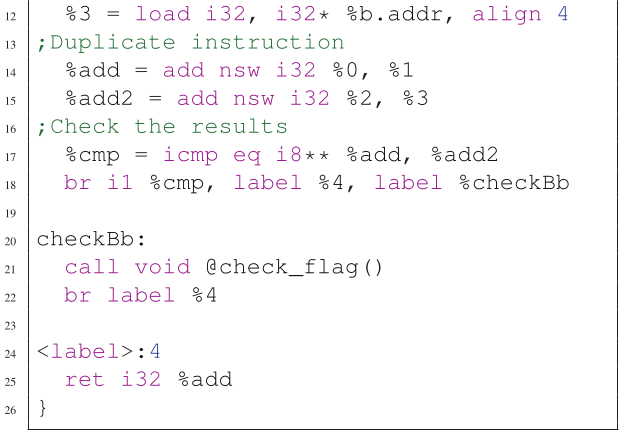
\includegraphics[width=1\linewidth]{img3.png}
				\caption{(b)}
				\label{IR code examples of using EDDs(b)}
			\end{figure}
		\end{column}
		\end{columns}
\end{frame}


%------------------------------------------------

\section{Main Contribution}

\begin{frame}
	\frametitle{Main Contribution}
	
	\begin{enumerate}
		\item \textbf{Proposed Solution:}
		\begin{itemize}
			\item FERRUM: Optimized assembly-level EDDI.
			\item Enhancements: Utilizes SIMD and compiler optimizations.
			\item Improves: Fault coverage and performance.
		\end{itemize}
		
		
		\item \textbf{Key Findings \& Results:}
		\begin{itemize}
			\item 28\% gap in fault coverage (IR-level vs. assembly-level).
			\item 100\% fault coverage with FERRUM at assembly level.
			\item 52\% reduction in runtime overhead with FERRUM, no loss in fault coverage.
		\end{itemize}
	\end{enumerate}
	
	
	
	
	
	
	
%	\begin{columns}[c] % The "c" option specifies centered vertical alignment while the "t" option is used for top vertical alignment
%		\begin{column}{0.45\textwidth} % Left column width
%			\textbf{Heading}
%			\begin{enumerate}
%				\item Statement
%				\item Explanation
%				\item Example
%			\end{enumerate}
%		\end{column}
%		\begin{column}{0.5\textwidth} % Right column width
%			Lorem ipsum dolor sit amet, consectetur adipiscing elit. Integer lectus nisl, ultricies in feugiat rutrum, porttitor sit amet augue. Aliquam ut tortor mauris. Sed volutpat ante purus, quis accumsan dolor.
%		\end{column}
%	\end{columns}
\end{frame}

%------------------------------------------------

\section{Background}
\begin{frame}
	\frametitle{Background}
	\begin{enumerate}
		\item \textbf{Focus on single bit-flip transient faults in:}
		\begin{itemize}
			\item Processor computing components
			\item Pipeline stages
			\item Arithmetic components
			\item Load/store units
		\end{itemize}
		\textcolor{red}{Do not consider faults in the memory or caches, as we assume they have already been protected by ECC (Error Correcting Code).}
		
		\item \textbf{Fault Simulation:}
		Assembly-level fault injection; beam testing infeasible.
		
		\item \textbf{EDDI:}
		Instruction duplication, runtime comparison.
		
%		\item \textbf{Compilation:}
%		\begin{itemize}
%			\item IR-level: Common, uses LLVM tools.
%			\item Assembly-level: Rare, closer to hardware.
%		\end{itemize}
		
		\item \textbf{Platform:} x86 ISA (other platforms for future work).
	\end{enumerate}
\end{frame}





\section{FERRUM}
\subsection{High-Level Design}
\begin{frame}
	\frametitle{High-Level Design}
	
	% TODO: \usepackage{graphicx} required
	\begin{figure}
		\centering
		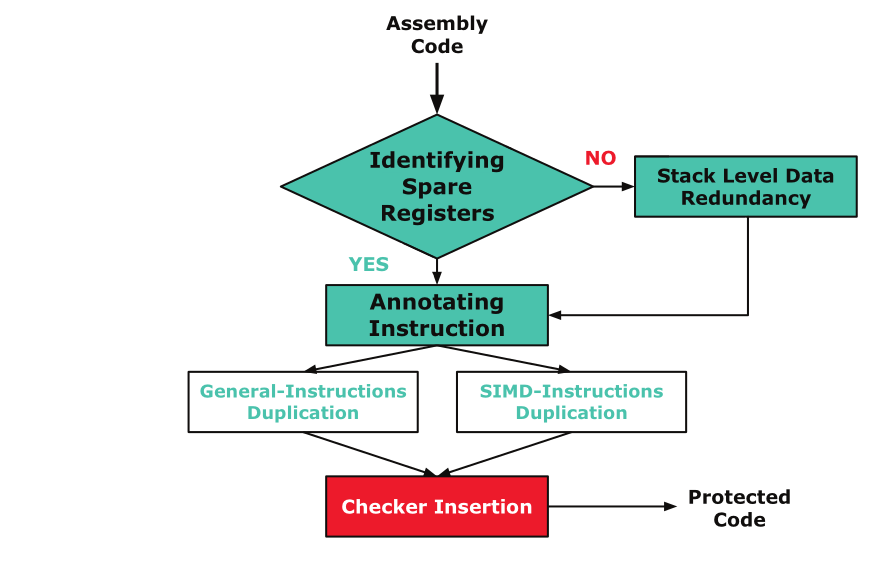
\includegraphics[width=0.7\linewidth]{Images/img10}
		\label{fig:img10}
	\end{figure}
	
		\begin{itemize}
			\item Scan registers (general-purpose, SIMD); identify spare registers.
			\item Annotate instructions for SIMD compatibility.
			\item Duplicate instructions; use SIMD or general-purpose registers.
		\end{itemize}
\end{frame}




\subsection{Components}
\begin{frame}
	\frametitle{Components}
	\begin{enumerate}
		\item \textbf{Static Code Analysis}
		\begin{itemize}
			\item Identify spare registers (general-purpose: 2, SIMD: 4 XMM).
			\item Annotate instructions (SIMD-enabled or general).	
		\end{itemize}
		
		\item \textbf{Duplication for General Instructions}
		\begin{itemize}
			\item Duplicate instructions; use spare registers or deferred detection for comparisons (e.g., \texttt{rflag}).
		\end{itemize}
		
		\item \textbf{Duplication for SIMD-Enabled Instructions}
		\begin{itemize}
			\item Use SIMD registers (e.g., XMM, YMM) for bulk comparison.
			
			\item Leverage architecture-specific features (e.g., ZMM on Intel CPUs).
		\end{itemize}
		
		
%		\item \textbf{Stack-Level Data Redundancy}
%		\begin{itemize}
%			\item Buffer unused registers onto stack when spare registers are insufficient.
%			\item Restore registers after duplication and checking.
%		\end{itemize}
		
		
		
%		\item \textbf{Other ISAs}
%		\begin{enumerate}
%			\item Potential for adaptation (e.g., ARM NEON, x86 AVX-512).
%			\item Future work includes exploring ISA-specific optimizations.
%		\end{enumerate}
	\end{enumerate}
\end{frame}






\begin{frame}
	\frametitle{Example1}
	
	% TODO: \usepackage{graphicx} required
	\begin{figure}
		\centering
		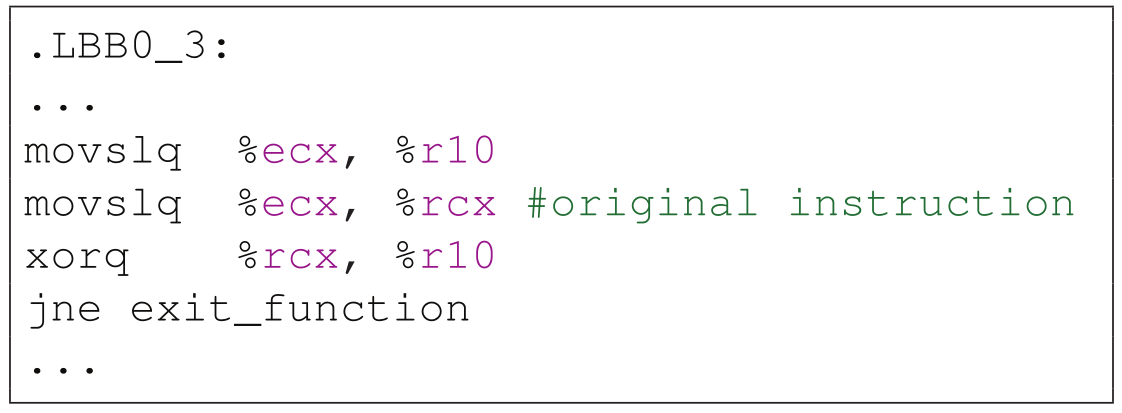
\includegraphics[width=0.8\linewidth]{Images/img11}
		\caption{Protection of GENERAL-INSTRUCTIONS (\texttt{movslq})}
		\label{fig:Protection of G ENERAL - INSTRUCTIONS}
	\end{figure}
	
\end{frame}


\begin{frame}
	\frametitle{Example2}
	
	% TODO: \usepackage{graphicx} required
	\begin{figure}
		\centering
		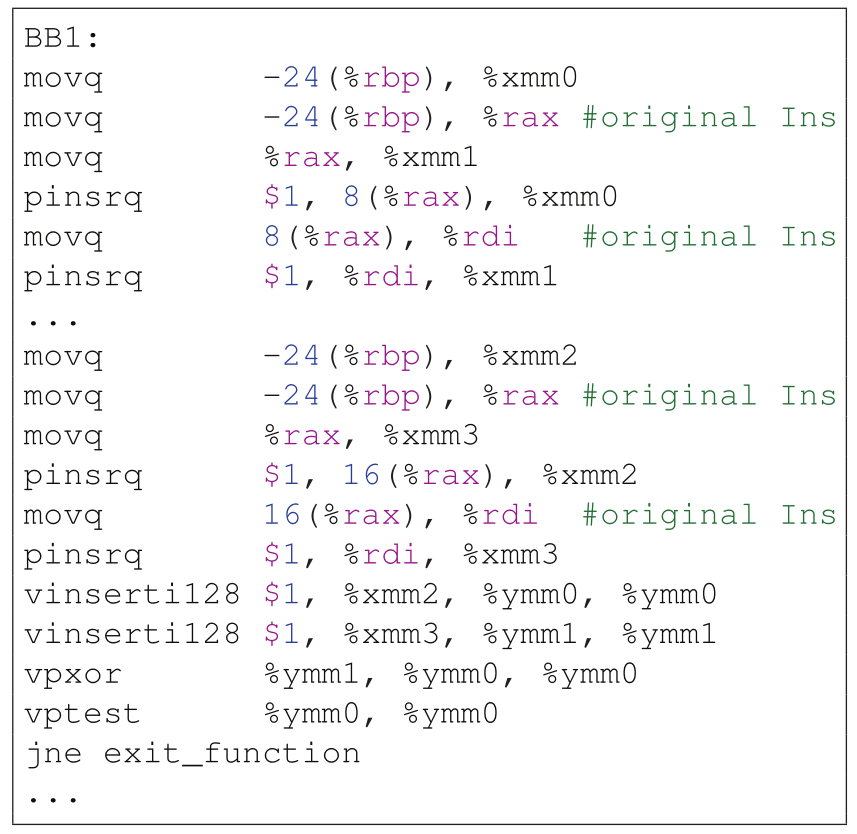
\includegraphics[width=0.6\linewidth]{Images/img12}
		\caption{FERRUM using SIMD capability}
		\label{fig:FERRUM using SIMD capability}
	\end{figure}
	
\end{frame}








\section{Evaluation}
\subsection{Experimental Setup}
\begin{frame}
	\frametitle{Experimental Setup}
	
	
	\begin{table}[h!]
		\centering
		\caption{Details of Benchmarks}
		\begin{tabular}{lll}
			\toprule
			\textbf{Benchmark} & \textbf{Suite} & \textbf{Domain} \\
			\midrule
			Backprop          & Rodinia        & Machine Learning       \\
			BFS               & Rodinia        & Graph Algorithm        \\
			Pathfinder        & Rodinia        & Dynamic Programming    \\
			LUD               & Rodinia        & Linear Algebra         \\
			Needle            & Rodinia        & Dynamic Programming    \\
			kNN               & Rodinia        & Machine Learning       \\
			kmeans            & Rodinia        & Data Mining            \\
			Particlefilter    & Rodinia        & Noise estimator        \\
			\bottomrule
		\end{tabular}
	\end{table}
	
	\begin{itemize}
		\item Platform: Ubuntu 20.04, Intel Xeon (x86-64), 64GB RAM.
	\end{itemize}
\end{frame}





\subsection{Fault Injection Methodology}
\begin{frame}
	\frametitle{Fault Injection Methodology}
	
	\begin{enumerate}
		\item \textbf{Single bit-flip faults} injected at assembly level.
		\item \textbf{1000 random faults} injected per benchmark.
	\end{enumerate}
	
	
	\begin{enumerate}
		\item \textbf{Metrics:}
		
		\begin{itemize}
			\item SDC Coverage: Measures reduction in Silent Data Corruptions. 
			% $$ Coverage = \frac{SDC_{raw} - SDC_{prot} }{SDC_{raw}} $$
			
			\item Runtime Overhead: Measures performance impact. 
			% $$ Overhead = \frac{Runtime_{prot} - Runtime_{raw} }{Runtime_{raw}} $$
			
			\item FERRUM Execution Time: Compile-time overhead.

		\end{itemize}
	\end{enumerate}
\end{frame}





%\subsection{Key Observations}
%\begin{frame}
%	\frametitle{Key Observations}
%	
%	
%	
%	\begin{table}[h!]
%		\centering
%		\caption{FERRUM and Baseline Techniques}
%		\resizebox{\textwidth}{!}{%
%			\begin{tabular}{lcccccc}
%				\toprule
%				\textbf{} & \textbf{basic} & \textbf{store} & \textbf{branch} & \textbf{call} & \textbf{mapping} & \textbf{comparison} \\
%				\midrule
%				IR-level-EDDI                 & \textit{IR} & / & / & / & / & / \\
%				Hybrid-assembly-level-EDDI    & \textit{AS$_1$} & \textit{AS$_1$} & \textit{IR} & \textit{AS$_1$} & \textit{AS$_1$} & \textit{IR} \\
%				FERRUM                        & \textit{AS$_2$} & \textit{AS$_2$} & \textit{AS$_2$} & \textit{AS$_2$} & \textit{AS$_2$} & \textit{AS$_2$} \\
%				\bottomrule
%			\end{tabular}%
%		}
%	\end{table}
%	
%	
%\end{frame}



%\begin{frame}
%	\frametitle{Table}
%	\framesubtitle{Subtitle} % Optional subtitle
%	
%	\begin{table}
%		\begin{tabular}{l l l}
%			\toprule
%			\textbf{Treatments} & \textbf{Response 1} & \textbf{Response 2}\\
%			\midrule
%			Treatment 1 & 0.0003262 & 0.562 \\
%			Treatment 2 & 0.0015681 & 0.910 \\
%			Treatment 3 & 0.0009271 & 0.296 \\
%			\bottomrule
%		\end{tabular}
%		\caption{Table caption}
%	\end{table}
%\end{frame}
%------------------------------------------------



%------------------------------------------------

\section{Results}
\subsection{SDC Coverage}

\begin{frame}
	\frametitle{SDC Coverage}
	
	\begin{figure}
		\centering
		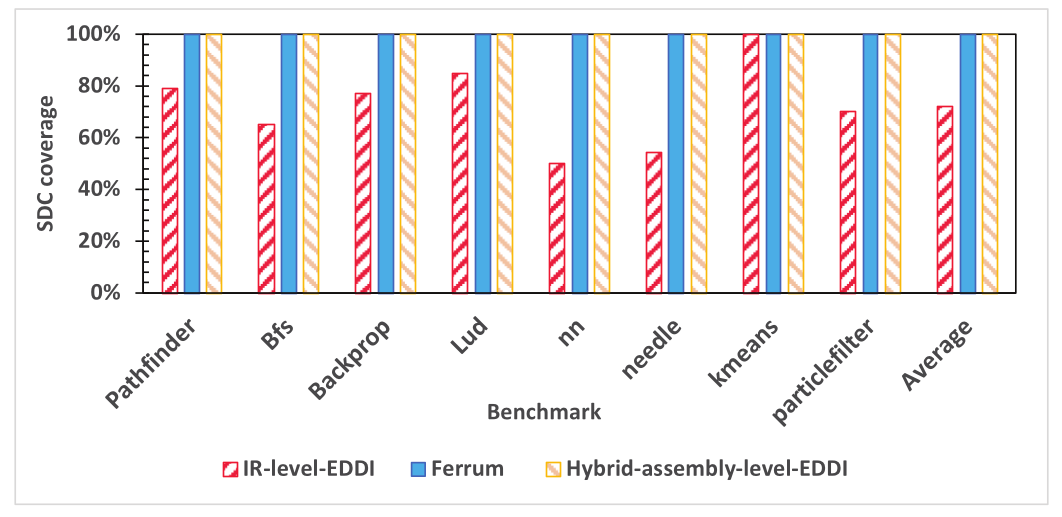
\includegraphics[width=1\linewidth]{img7.png}
		\caption{SDC coverage measured}
		\label{SDC coverage measured}
	\end{figure}
\end{frame}




\subsection{Runtime Performance Overhead}
\begin{frame}
	\frametitle{Runtime Performance Overhead}
	
	\begin{figure}
		\centering
		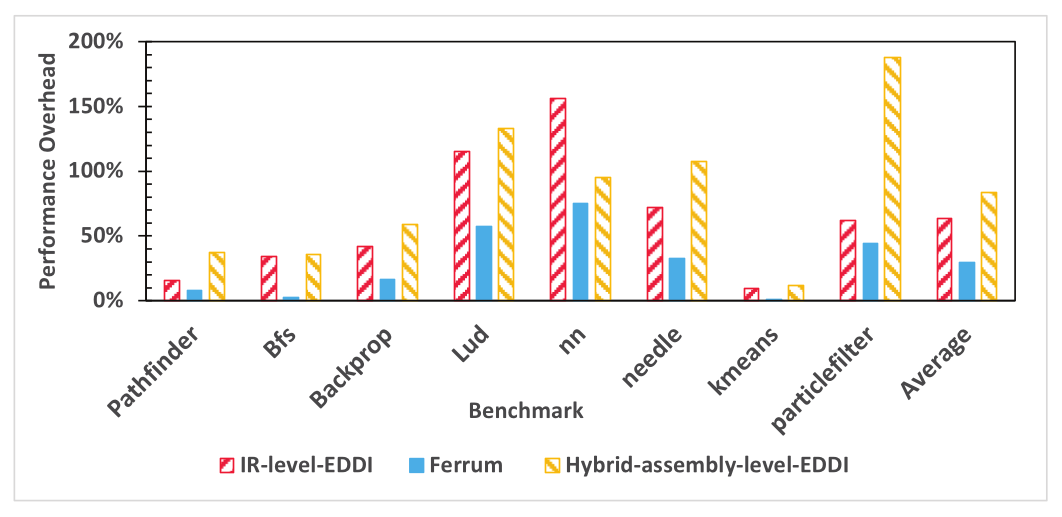
\includegraphics[width=1\linewidth]{img9.png}
		\caption{Performance overhead measured}
		\label{Performance overhead measured}
	\end{figure}
\end{frame}



\subsection{Execution Time}
\begin{frame}
	\frametitle{Execution Time}
	
	\begin{enumerate}
		\item Average: 0.117 seconds.
		\item Max: 0.196 seconds.
		\item Min: 0.089 seconds (BFS).
	\end{enumerate}
\end{frame}


%%------------------------------------------------
%
%\begin{frame}
%	\frametitle{Theorem, Corollary \& Proof}
%	
%	\begin{theorem}[Mass--energy equivalence]
%		$E = mc^2$
%	\end{theorem}
%	
%	\begin{corollary}
%		$x + y = y + x$
%	\end{corollary}
%	
%	\begin{proof}
%		$\omega + \phi = \epsilon$
%	\end{proof}
%\end{frame}
%
%%------------------------------------------------
%
%\begin{frame}
%	\frametitle{Equation}
%
%	\begin{equation}
%		\cos^3 \theta =\frac{1}{4}\cos\theta+\frac{3}{4}\cos 3\theta
%	\end{equation}
%\end{frame}
%
%%------------------------------------------------
%
%\begin{frame}[fragile] % Need to use the fragile option when verbatim is used in the slide
%	\frametitle{Verbatim}
%	
%	\begin{example}[Theorem Slide Code]
%		\begin{verbatim}
%			\begin{frame}
%				\frametitle{Theorem}
%				\begin{theorem}[Mass--energy equivalence]
%					$E = mc^2$
%				\end{theorem}
%		\end{frame}\end{verbatim} % Must be on the same line
%	\end{example}
%\end{frame}
%
%%------------------------------------------------
%
%\begin{frame}
%	Slide without title.
%\end{frame}
%
%%------------------------------------------------
%
%\section{Referencing}
%
%\begin{frame}
%	\frametitle{Citing References}
%	
%	An example of the \texttt{\textbackslash cite} command to cite within the presentation:
%	
%	\bigskip % Vertical whitespace
%	
%	This statement requires citation \cite{p1,p2}.
%\end{frame}

%------------------------------------------------

\begin{frame} % Use [allowframebreaks] to allow automatic splitting across slides if the content is too long
	\frametitle{References}
	
	\begin{thebibliography}{99} % Beamer does not support BibTeX so references must be inserted manually as below, you may need to use multiple columns and/or reduce the font size further if you have many references
		\footnotesize % Reduce the font size in the bibliography
		
		\bibitem[He et al., 2024]{p1}
			Zhengyang He, Hui Xu, Guanpeng Li (2024)
			\newblock A Fast Low-Level Error Detection Technique
			\newblock \emph{2024 54th Annual IEEE/IFIP International Conference on Dependable Systems and Networks (DSN)}, University of Iowa, Iowa City, IA, USA; Fudan University, Shanghai, China.
		
		
	\end{thebibliography}
\end{frame}

%----------------------------------------------------------------------------------------
%	ACKNOWLEDGMENTS SLIDE
%----------------------------------------------------------------------------------------

%\begin{frame}
%	\frametitle{Acknowledgements}
%	
%	\begin{columns}[t] % The "c" option specifies centered vertical alignment while the "t" option is used for top vertical alignment
%		\begin{column}{0.45\textwidth} % Left column width
%			\textbf{Smith Lab}
%			\begin{itemize}
%				\item Alice Smith
%				\item Devon Brown
%			\end{itemize}
%			\textbf{Cook Lab}
%			\begin{itemize}
%				\item Margaret
%				\item Jennifer
%				\item Yuan
%			\end{itemize}
%		\end{column}		
%		\begin{column}{0.5\textwidth} % Right column width
%			\textbf{Funding}
%			\begin{itemize}
%				\item British Royal Navy
%				\item Norwegian Government
%			\end{itemize}
%		\end{column}
%	\end{columns}
%\end{frame}

%----------------------------------------------------------------------------------------
%	CLOSING SLIDE
%----------------------------------------------------------------------------------------

\begin{frame}[plain] % The optional argument 'plain' hides the headline and footline
	\begin{center}
		{\Huge The End}
		
		\bigskip\bigskip % Vertical whitespace
		
		{\LARGE Questions? Comments?}\vfil
		\texttt{\href{mailto:adinepour@aut.ac.ir}{\textcolor{red}{adinepour@aut.ac.ir}}}
	\end{center}
\end{frame}

%----------------------------------------------------------------------------------------

\end{document} 